\documentclass[a4paper,10pt]{article}
\usepackage{amsmath}
\usepackage{geometry}
\usepackage{bm}
\usepackage{graphicx}
\geometry{left=1.25cm,right=1.25cm,top=2cm,bottom=2cm}
\begin{document}
12132386 Chen Yujie
\begin{center}
\LARGE \textbf {Project Report}\\
{\large one-dimensional heat conduction}
\\ \hspace*{\fill} \\
\end{center}

\large \textbf {Algorithm framework}

In this project, the governing equation of one-dimensional heat conduction problem, the boundary conditions and the initial value can be expressed as
\begin{align}
\rho c\frac{\partial u}{\partial t}-\kappa \frac{\partial ^2 u}{\partial x^2}=f \quad &on\  \Omega \times (0,T) \\
u=0 \quad &on \  \Gamma \times (0,T) \\
u|_{t=0} =u_0 =  e^x \quad &in \ \Omega .
\end{align}
Here, $\Omega$ :=(0,1) is the 1D domain. The boundary domain is $\Gamma$ = $\left\{ 0,1 \right\} $. $\rho$, $c$, $\kappa$ are the density, heat capacity and heat conductivity respectively. $f \ =sin(\pi x)$ is the heat supply per unit volume. 

Both explicit and implicit method is applied to solve this problem. The derivation of the two schemes are provided as follows.

Explicit Euler method
\begin{align*}
& \rho c \frac{\partial u}{\partial t} - \kappa \frac{\partial ^2 u}{\partial x^2} = f \\
& \frac{\partial u}{\partial t} = \frac{\kappa}{\rho c} \frac{\partial ^2 u}{\partial x^2} + \frac{f}{\rho c} \\
& \frac{\partial u}{\partial t} \sim \frac{U_i^{n+1} - U_i^n}{\Delta t} \\
& \frac{\partial ^2 u}{\partial x^2} \sim \frac{U_{i-1}^n - 2 U_i^n + U_{i+1}^n}{\Delta x^2} \\
& \frac{U_i^{n+1} - U_i^n}{\Delta t} = \frac{\kappa}{\rho c} \frac{U_{i-1}^n - 2 U_i^n + U_{i+1}^n}{\Delta x^2} + \frac{f}{\rho c} \\
& U_i^{n+1} - U_i^n = \frac{\kappa \Delta t}{\rho c \Delta x^2} ( U_{i-1}^n - 2 U_i^n + U_{i+1}^n ) + \frac{f \Delta t}{\rho c} \\
& U_i^{n+1} = \frac{\kappa \Delta t}{\rho c \Delta x^2} U_{i-1}^n + ( 1 - 2 \frac{\kappa \Delta t}{\rho c \Delta x^2} ) U_i^n + \frac{\kappa \Delta t}{\rho c \Delta x^2} U_{i+1}^n + \frac{f \Delta t}{\rho c} \\
& \bm A = \bm I + \frac{\kappa \Delta t}{\rho c \Delta x^2}
\begin{bmatrix}
-2 & 1  & \  & \  & \  \\
1  & -2 & 1  & \  & \  \\
\  & \ddots & \ddots & \ddots & \ \\
\  & \  & 1  & -2 & 1  \\
\  & \  & \  & 1  & -2 
\end{bmatrix} \\
& \bm U^{n+1} = \bm A \bm U^n
\end{align*}

Implicit Euler method
\begin{align*}
& \rho c \frac{\partial u}{\partial t} - \kappa \frac{\partial ^2 u}{\partial x^2} = f \\
& \frac{\partial u}{\partial t} = \frac{\kappa}{\rho c} \frac{\partial ^2 u}{\partial x^2} + \frac{f}{\rho c} \\
& \frac{\partial u}{\partial t} \sim \frac{U_i^{n+1} - U_i^n}{\Delta t} \\
& \frac{\partial ^2 u}{\partial x^2} \sim \frac{U_{i-1}^{n+1} - 2 U_i^{n+1} + U_{i+1}^{n+1}}{\Delta x^2} \\
& \frac{U_i^{n+1} - U_i^n}{\Delta t} = \frac{\kappa}{\rho c} \frac{U_{i-1}^{n+1} - 2 U_i^{n+1} + U_{i+1}^{n+1}}{\Delta x^2} + \frac{f}{\rho c} \\
& U_i^{n+1} - U_i^n = \frac{\kappa \Delta t}{\rho c \Delta x^2} \left( U_{i-1}^{n+1} - 2 U_i^{n+1} + U_{i+1}^{n+1} \right) + \frac{f \Delta t}{\rho c} \\
& - \frac{\kappa \Delta t}{\rho c \Delta x^2} U_{i+1}^{n+1} + \left( 1 + 2 \frac{\kappa \Delta t}{\rho c \Delta x^2} \right) U_i^{n+1} - \frac{\kappa \Delta t}{\rho c \Delta x^2} U_{i-1}^{n+1} = U_i^n + \frac{f \Delta t}{\rho c} \\
& \bm A = \bm I + \frac{\kappa \Delta t}{\rho c \Delta x^2}
\begin{bmatrix}
2  & -1 & \  & \  & \  \\
-1 & 2  & -1 & \  & \  \\
\  & \ddots & \ddots & \ddots & \ \\
\  & \  & -1 & 2  & -1 \\
\  & \  & \  & -1 & 2 
\end{bmatrix} \\
& \bm A \bm U^{n+1} = \bm U^n
\end{align*}

The convergence condition for explicit scheme is 
\begin{align*}
\frac{\kappa \Delta t}{\rho c \Delta x^2} < \frac{1}{2},
\end{align*}
and the implicit scheme always converges.

The steady state is characterized by $\partial u/ \partial t=0$. Thus, $u=\frac{sin(\pi x)}{\pi ^2}$ at steady state.\\

\large \textbf {Error Analysis}

Here, I focused on the value at the center of the domain, i.e. at x=0.5. In explicit scheme, the error of the data is related to the discretization of space and time: 
\begin{align}
e \approx C_1 \Delta x^\alpha + C_2 \Delta t^\beta .
\end{align}

To get the value of $\alpha$ , $\Delta$ t is fixed at 5e-6, and the domain is divided into 8, 16, 32, 64, 128, 256 parts respectively. The value of $u$ changes little after 1.5 seconds, i.e., the steady state is roughly after 1.5 seconds. In this part, the iteration number is set 400000 to stop after 2 seconds. The corresponding error is defined as the difference between the numerical data and the theoretical data at x=0.5. Note that the theoretical data at x=0.5 at steady state is $1/(\pi ^2)$. The results are plot is log form. As shown in Fig. 1, the slop of the line is around 2.001. Thus, the value of $\alpha$ is determined as 2.
\begin{figure}[h]
	\centering
	\includegraphics[scale=1]{alpha.eps}
	\caption{err versus dx}
\end{figure}

To get the value of $\beta$, $\Delta x$ is fixed at 0.005, $\Delta t$ varies at 1e-6, 5e-6, 2.5e-6, 1.25e-6, 6.25e-7, 3.125e-7. Each sample stop at 0.1 second. The error is defined as the difference between each sample at the sample of $\Delta t = 3.125e-7$. The results are plot in log form. As shown in Fig. 2, the slop of the line passing through the red points is 0.94. Thus, the value of $\beta$ is determined as 1.
\begin{figure}[h]
	\centering
	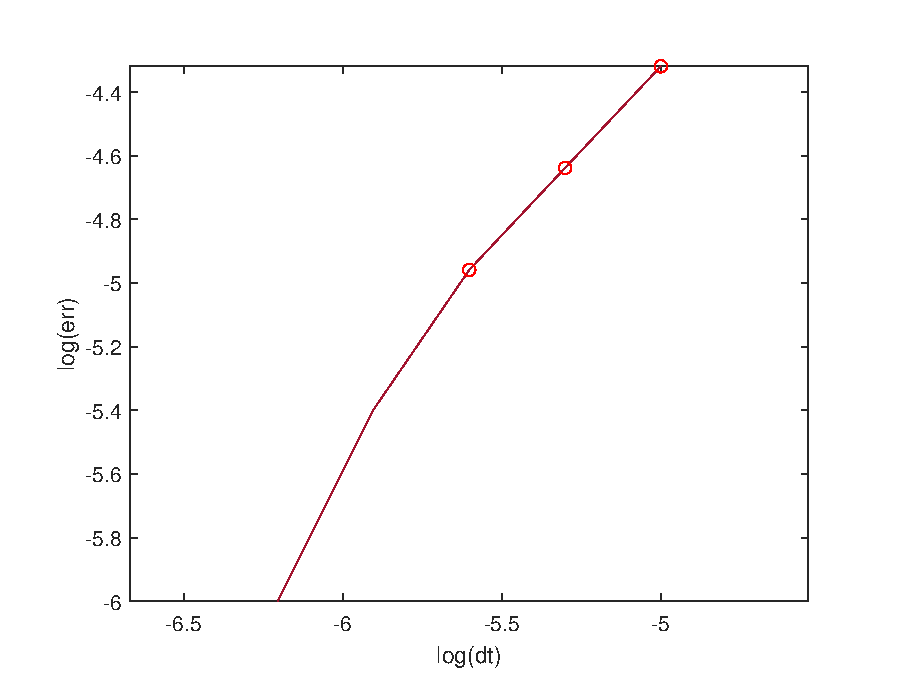
\includegraphics[scale=1]{beta.eps}
	\caption{err versus dt}
\end{figure}

\clearpage

\large \textbf {Parallelism}

In this part, examples of parallel behaviours are presented from explicit scheme. To observe Amdahl's Law, the domain is divided into 40000 parts, and the processor number is set 1, 2, 4, 8 respectively. Fig. 3 shows the speed-up ratio with respect to processor number. The yellow line has a slope of 1 for reference. 
\begin{figure}[h]
	\centering
	\includegraphics[scale=0.6]{Amdahl.png}
	\caption{speed-up ratio versus processor number}
\end{figure} \\

To observe Gustafson's Law, division number is set 500, 1000, 1500, 2000, 2500, 3000 with processor number at 1, 4, 9, 16, 27, 36 respectively. Fig. 4 illustrates the time spent with respect to processor number. Time spent increase gradually as processor number increases. While the time cost using 4 processors is significant higher abnormally, which needs further discussion. 
\begin{figure}[h]
	\centering
	\includegraphics[scale=0.6]{Gustafson.png}
	\caption{time spent versus processor number}
\end{figure} \\
\clearpage

\large \textbf {Visualization}

To visualize the results, output data is written in tecplot manner. Fig. 5 is from implicit scheme with matrix size of 1000 by 1000. 
\begin{figure}[h]
	\centering
	\includegraphics[scale=0.2]{result_in_tecplot.png}
	\caption{result shown by tecplot. X is the coordinate}
\end{figure} \\
























\end{document}